%  !TeX  root  =  user_guide.tex
\chapter{Lavorare con i dati OGC}\label{working_with_ogc}

% when the revision of a section has been finalized,
% comment out the following line:
% \updatedisclaimer

QGIS supporta sorgenti di dati WMS e WFS. Il supporto WMS è nativo, quello per
WFS e WFS-T è fornito tramite plugin.

\section{Cosa sono i dati OGC}\index{OGC!introduzione}

L'Open Geospatial Consortium (OGC), è un'organizzazione internazionale che raggruppa più
di 300 organizzazioni commerciali, governative, nonprofit e di ricerca.
I suoi membri sviluppano e implementano standard per contenuti e servizi geospaziali,
analisi GIS e scambio dati.

OGC ha elaborato un numero crescente di specifiche per la descrizione di un modello dati di base 
per elementi geografici: le specifiche sono orientate a garantire l'interoperabilità
nell'ambito della tecnologia geospaziale. Ulteriori informazioni all'indirizzo \url{http://www.opengeospatial.org/}.

Importanti specifiche OGC sono:

\begin{itemize}[label=--]
\item \textbf{WMS} - Web Map Service
\item \textbf{WFS} - Web Feature Service
\item \textbf{WCS} - Web Coverage Service
\item \textbf{CAT} - Web Catalog Service
\item \textbf{SFS} - Simple Features for SQL
\item \textbf{GML} - Geography Markup Language
\end{itemize}

Ad oggi i servizi OGC-sono sempre più di uso comune per scambiare dati geografici fra
differenti implementazioni GIS. QGIS ora può gestire tre delle specifiche esposte sopra, 
SFS (tramite il supporto a PostgreSQL/PostGIS, vedi Sezione \ref{label_postgis}), WFS e WMS come client.

\section{Client WMS}\label{sec:ogc-wms}\index{WMS!client}\index{OGC!WMS!client}\index{raster!WMS}

\subsection{Panoramica sul servizio WMS}\label{sec:ogc-wms-about}\index{WMS!client!considerazioni}

QGIS può agire come client WMS, nel rispetto delle specifiche 1.1, 1.1.1 e 1.3.
È stato particolarmente testato nei confronti di server accessibili pubblicamente
quali DEMIS e JPL OnEarth.

I server WMS rispondono alle richieste da parte dei client (ad es. QGIS) di una mappa raster
di una determinata estensione, con un determinato insieme di layer, simboli e trasparenze.
Il server WMS quindi consulta le sue risorse (locali o remote), genera il raster e lo invia
al client in formato raster, per QGIS tipicamente come immagini JPEG o PNG.

WMS è un servizio REST (Representational State Transfer) piuttosto che un servizio web completo.
Come tale, si può prendere l'URL (indirizzo del server con specifiche) generato da QGIS e usarlo
in un browser web per ottenere la stessa immagine che QGIS usa internamente. Questo può essere
utile per identificare le cause di eventuali problemi, dato che esistono vari tipi di server
WMS e ciascuno ha la sua propria interpretazione degli standard WMS.

I layer WMS possono essere aggiunti molto semplicemente, una volta
disponibile l'indirizzo (URL) per accedere al server WMS, una connessione adatta
e posto che il server usi HTTP come meccanismo di trasferimento dati.

\subsection{Selezionare un server WMS}\label{sec:ogc-wms-servers}\index{WMS!server remoto!selezionare}

Al primo utilizzo di un servizio WMS in QGIS non sono presenti
server predefiniti. Si può avviare lo strumento cliccando sul pulsante
\toolbtntwo{mActionAddWmsLayer}{Aggiungi layer WMS} nella barra strumenti, 
oppure sulla voce di menu
\mainmenuopt{Layer} \arrow \dropmenuopttwo{mActionAddWmsLayer}{Aggiungi layer WMS...}.
Si aprirà la finestra di dialogo \dialog{Aggiungi layer dal server}. È
possibile aggiungere alcuni server cliccando sul pulsante
\button{Aggiungere server predefiniti}. Verranno quindi aggiunti almeno tre
server WMS, incluso il server della NASA (JPL). Per definire un nuovo server WMS
nella sezione \tab{Layer}, cliccare su \button{Nuovo} ed inserire
i parametri di connessione al server WMS desiderato, seguendo le indicazioni della
tabella \ref{tab:wms_connection_parms}:

\begin{table}[ht]\index{WMS!client!parametri di connessione}
\centering
 \begin{tabular}{|l|p{11cm}|}
\hline Nome & Un nome per connessione. \\
\hline URL \index{WMS!URL} & URL del server che fornisce i dati.
 Deve essere un indirizzo raggiungibile nello stesso formato che verrebbe usato
 per aprire una commessione telnet o pingare un host. \\
\hline Username \index{WMS!autenticazione} & Nome utente per accedere
 un WMS protetto. Questo parametro è opzionale. \\
\hline Password & Password per accedere ad un WMS protetto. 
 Questo parametro è opzionale.\\
\hline Ignora URI GetMap & \checkbox{Ignora la URI GetMap 
riportata nelle capabilities}. Viene utilizzato URI del campo URL precedente\\
\hline Ignora URI GetFeatureInfo & \checkbox{Ignora la URI GetFeatureInfo
riportata nelle capabilities}. Viene utilizzato URI del campo URL precedente\\
\hline
\end{tabular}
\caption{Parametri di connessione WMS}\label{tab:wms_connection_parms}
\end{table}

È possibile, se necessario, impostare i parametri di un proxy per ricevere i servizi WMS da internet.
Selezionare la voce di menu \mainmenuopt{Impostazioni} \arrow \dropmenuopttwo{mActionOptions}{Opzioni} e cliccare sulla scheda
\tab{Rete}, nella quale è possibile inserire le impostazioni abilitando la
casella di controllo \checkbox{Utilizza un proxy per l'accesso web}.

Una volta creata la connessione al server WMS, essa sarà memorizzata e
disponibile per le successive sessioni di QGIS.

\begin{Tip}[ht]\caption{\textsc{A proposito di indirizzi dei server WMS}}
Quando si inserisce l'indirizzo URL del server assicurarsi di
usare l'indirizzo di base. Ad esempio non bisogna inserire frammenti tipo
\usertext{request=GetCapabilities} o \usertext{version=1.0.0} nell'indirizzo.\index{WMS!server remoto!URL}
\end{Tip}

\subsection{Caricare layer WMS}\label{sec:ogc-wms-layers}\index{WMS!client!layer}

Una volta compilati correttamente i campi, si può premere sul pulsante
\button{Connetti} per ottenere le \textit{capabilities} del server: in esse sono inclusi
i formati immagine, i layer disponibili e i sistemi di proiezione forniti dal
server. Considerato che si tratta di operazioni in rete, la velocità nella
risposta dipenderà dalla qualità della connessione verso il server WMS. Mentre
si scaricano i dati dal server, l'avanzamento dell'operazione viene
visualizzato nella porzione inferiore sinistra della finestra. 

\begin{figure}[ht]
  \centering
  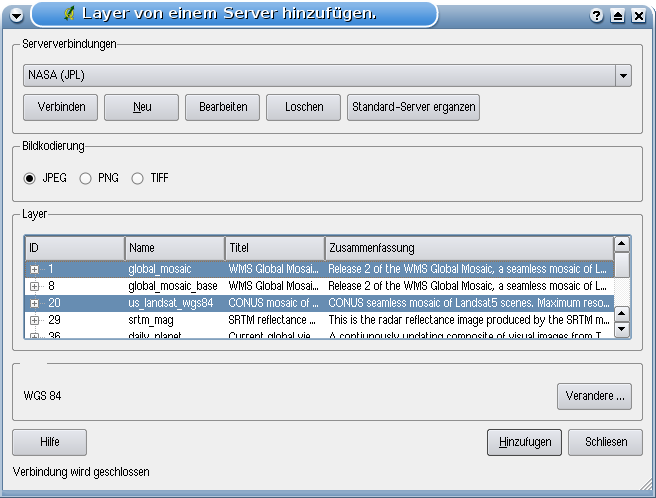
\includegraphics[clip=true,width=0.6\textwidth]{connection_wms}
  \caption{Finestra di dialogo per l'aggiunta di un server WMS \nixcaption}\label{fig:connection_wms}
\end{figure}

\minisec{Codifica immagine}

La sezione \tab{Codifica immagine} elenca i formati supportati sia dal client
che dal  server. La scelta è in funzione dei propri requisiti di accuratezza.

\begin{Tip}[ht]\caption{\textsc{Codifica immagine}}
Solitamente un server WMS offrirà la scelta tra le codifiche JPEG e
PNG. Mentre la compressione JPEG comporta una perdita di qualità, quella PNG
riproduce fedelmente il dato di origine. Usare JPEG se non interessa avere una
certa perdita di qualità dell'immagine, riducendo d'altro canto il tempo per
il download dei dati di 5 volte rispetto al formato PNG. Usare invece PNG se
si vuole una rappresentazione precisa del dato originale e non ci si preoccupa
del tempo necessario per il trasferimento dei dati.
\index{WMS!codifica immagine}
\end{Tip}

\minisec{Opzioni}

La sezione Opzioni mette a disposizione il campo testo Nome layer per associare un nome al layer WMS: 
tale nome apparirà nella legenda a caricamento avvenuto. 

Sotto Nome layer appare il sistema di riferimento predefinito del server WMS. 
Se il pulsante \button{Cambia\dots} è attivo, allora è possibile selezionare un altro SR fornito dal server.

\begin{Tip}[ht]\caption{\textsc{Ordine dei layer WMS}}
In questa versione di QGIS, i layer WMS caricati sono sovrapposti in
base all'ordine in cui sono elencati nella sezione Layer, dall'alto verso il
basso. Se si desidera cambiare l'ordine di visualizzazione, usare la scheda \tab{Ordine layer}.
\index{WMS!server remoto!ordinamento layer}
\end{Tip}

\minisec{Trasparenza}\label{ogc-wms-transparency}

In questa versione di QGIS la trasparenza è impostata per essere sempre
attiva, se disponibile.

\begin{Tip}[ht]\caption{\textsc{Trasparenza dei Layer WMS}}
La possibilità di rendere trasparenti i layer WMS dipende dalla codifica 
tramite la quale sono stati caricati: PNG e GIF gestiscono la trasparenza mentre il JPEG no.
\index{WMS!trasparenza layer}
\end{Tip}

\minisec{Sistema di Riferimento}
\index{WMS!SR}\index{WMS!sistema di riferimento}
\index{OGC!SR}\index{OGC!sistema di riferimento}
\index{proiezioni!WMS}
\index{proiezioni!SR}\index{proiezioni!sistema di riferimento}
\index{SR}\index{sistema di riferimento}
\index{SR}\index{proiezioni!SR}

Sistema di riferimento delle coordinate (Coordinate Reference System) è
il termine OGC per una proiezione in QGIS.

Ogni layer WMS può essere restituito in molteplici SR, in funzione delle
capacità del server. Si noti che il numero di sistemi di riferimento tra cui
scegliere viene indicato nella dicitura \textsl{Sistemi di
Riferimento (x disponibili)} quando si seleziona/deseleziona un livello nella
sezione \tab{Layer}.

Per scegliere uno dei SR disponibili, cliccare su \button{Cambia...} per fare
apparire una finestra simile a quella della Figura \ref{fig:projections} alla
Sezione \ref{label_projstart}.
La differenza principale è che saranno mostrati solo i SR supportati dal server 
al quale si è connessi.

\begin{Tip}[ht]\caption{\textsc{Le proiezioni WMS}}
Per ottenere i migliori risultati, aggiungere per primo al progetto
il layer WMS, in modo che il sistema di riferimento dell'intero progetto sia
lo stesso attribuito al layer WMS.
Si potrà quindi usare la riproiezione al volo (Sezione \ref{sec:projection-specifying})
per adattare qualunque altro layer vettoriale successivamente aggiunto.
In questa versione di QGIS, aggiungere layer WMS successivamente ad altri e
con un SR diverso rispetto a quello del progetto, può causare errori.
\end{Tip}

\subsection{Cercare un Server}
\label{sec:serversearch}
\index{WMS!cerca server}
\index{WMS!ricerca}
\index{OGC!ricerca}

Con QGIS è anche possibile ricercare server WMS. La Figura \ref{fig:searchtab} mostra la nuova scheda 
\tab{Cerca Server} della finestra di dialogo \dialog{Aggiungi layer dal server}.

\begin{figure}[ht]
  \centering
  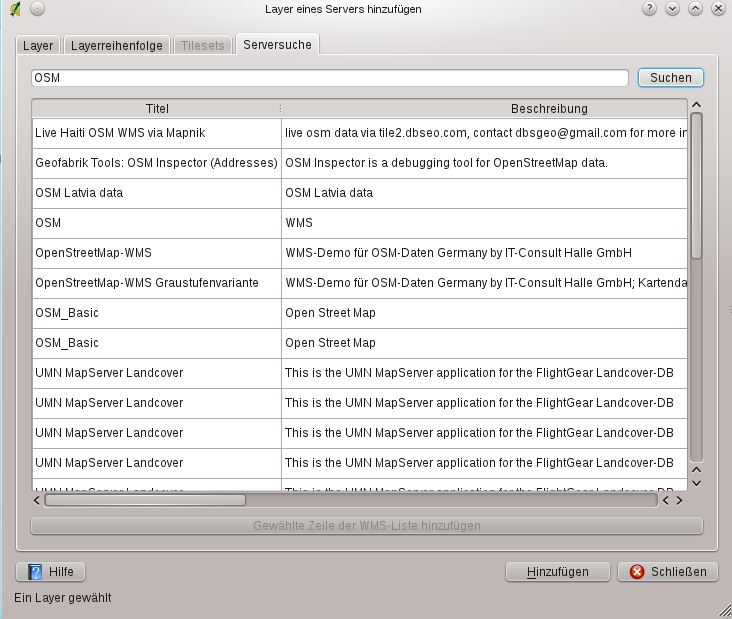
\includegraphics[clip=true,width=0.6\textwidth]{wms_server-search}
  	\caption{Ricerca server WMS \nixcaption}\label{fig:searchtab}
\end{figure}

Inserire una stringa di ricerca e cliccare sul pulsante \button{Cerca}: i risultati saranno elencati nella
sottostante tabella.

Per utilizzare uno dei risultati, selezionarlo nella tabella e cliccare su \button{Aggiungi riga alla lista WMS}. 
Il server verrà automaticamente aggiunto alla lista dei server nella scheda \tab{Layer}; cliccare su \button{Connetti} 
per ottenere la lista di layer forniti dal server.

Tale opzione, che è fondamentalmente un frontend alle API of \url{http://geopole.org}, 
è molto utile quando si vuole cercare una mappa in funzione di una parola chiave.

%
% Layer Order
%
\subsection{Ordine layer} \label{sec:layerorder}
\index{WMS!ordine layer}

Nella scheda \tab{Ordine layer} è possibile definire l'ordine di visualizzazione dei layer WMS, opzione utile
se si è selezionato un lungo elenco di layer e se ne vuole modificare l'ordine di sovrapposizione.

Selezionare il layer di interesse ed utilizzare le frecce su/giù per spostarlo nel posto desiderato.

%
% Tilesets
%
\subsection{Set di tile}\label{sec:tilesets}
\index{WMS!set di tilet}
\index{WMS!WMS-C}

Quando si usa un servizio WMS-C (Cached WMS) come ad esempio \url{http://labs.metacarta.com/wms-c/Basic.py}, 
si attiva la scheda \tab{Set di tile}, che fornisce informazioni sulle dimensione, il formato ed il SR dei tile.
In combinazione con tale opzione è possibile utilizzare la voce di menu 
\mainmenuopt{Visualizza} \arrow \dropmenuopt{Slider per la scala delle tiles}, che mette a disposizione le scale 
fornite dal server di tile.

\subsection{Uso dello strumento di identificazione}\label{sec:ogc-wms-identify}
\index{WMS!identificazione}
\index{identificazione!WMS}
\index{WMS!GetFeatureInfo}

Una volta aggiunto un server WMS, e se uno dei layer disponibili è
interrogabile, è possibile usare lo strumento
\toolbtntwo{mActionIdentify}{Informazioni elementi} per selezionare un pixel
sulla mappa, determinando una interrogazione verso il server WMS.

I risultati dell'interrogazione vengono restituiti come testo semplice la cui
formattazione dipenderà dalle impostazioni del server WMS.

\subsection{Proprietà del server}\label{sec:ogc-wms-properties}\index{WMS!proprietà}
\index{raster!proprietà}

Una volta aggiunto un server WMS, è possibile visualizzarne le proprietà
cliccando con il tasto destro sul suo nome nella legenda e selezionando
\button{Proprietà}.


\minisec{Scheda Metadati}\label{sec:ogc-wms-properties-metadata}
\index{raster!metadati}
\index{WMS!metadati}
\index{WMS!capabilities}

La scheda \tab{Metadati} mostra molte informazioni sul server WMS: tali informazioni sono fornite dal server stesso 
in risposta alla richiesta di "GetCapabilities" fatta da QGIS quando si connette ad esso.

Molte definizioni possono essere dedotte leggendo gli standard WMS \cite{OGCWMS010101web}, \cite{OGCWMS010300web}. 
Qui seguono alcune definizioni utili:

\begin{itemize}[label=--]
\item \textbf{Proprietà del server}

\begin{itemize}[label=--]
\item \textbf{Versione WMS}      - La versione WMS supportata dal server.

\item \textbf{Formati immagine}  - Elenco dei tipi MIME che il server può
                                   fornire  per disegnare la mappa. QGIS
				   supporta qualunque formato sia supportato
				   dalle librerie Qt contro le quali è
				   compilato, che sono solitamente almeno \texttt{image/png}
				   e \texttt{image/jpeg}.

\item \textbf{Interroga formati} - L'elenco dei tipi MIME con i quali il server
                                   può fornire risposta quando si usa lo strumento
				   "Informazioni elementi". Attualmente QGIS supporta
				   il tipo \texttt{text-plain}.

\end{itemize}

\item \textbf{Proprietà layer}

\begin{itemize}[label=--]
\item \textbf{Selezionato}         - Indica se il layer era selezionato quando
                                     il server è stato aggiunto al progetto.

\item \textbf{Visibilità}          - Indica se il layer è stato impostato
                                     come visibile in legenda.  (funzione non ancora utilizzata
				     in questa versione di QGIS.)

\item \textbf{Può interrogare}     - Indica se il layer fornisce o meno
                                     informazioni se si usa lo strumento "Informazioni elementi".

\item \textbf{Può essere trasparente} - Indica se il layer può essere o meno
                                        reso trasparente a video. Questa
					versione di QGIS farà sempre uso della
					trasparenza se questa voce visualizza
					\textsl{Sì} e se il formato immagine
					la supporta.
% BM: doesn't seem to work?
%                                    (see Section
%                                    \ref{ogc-wms-transparency}
%                                    ).

\item \textbf{Può ingrandire}      - Indica se il layer può o meno
                                     essere ingrandito dal server.
				     Questa versione di QGIS suppone che tutti i
                                     layer WMS abbiano questa opzione settata su \textsl{Sì}.
                                     Layers carenti in questa impostazione
				     potrebbero essere resi a video in modo
				     anomalo.

\item \textbf{Conteggio a cascata}    - I server WMS possono fungere da proxy
                                        per altri server WMS dai quali ottengono
					i dati raster per un certo layer. La
                                        voce mostra quindi quante richieste per questo
					layer vengono inoltrate ai nodi
                                        per ottenere un risultato.

\item \textbf{Larghezza fissa}, \textbf{Altezza fissa}
                                - Indica se il layer ha o meno una
				dimensione del pixel fissata alla sorgente.
                                  Questa versione di QGIS assume che tutti i
				  layer WMS abbiano vuota questa voce. Layers
				  con impostazioni diverse potrebbero essere resi
				  a video in modo anomalo.

\item \textbf{Perimetro WGS 84} - Estensione del layer in coordinate WGS84. Alcuni server
                                   WMS non settano questo parametro correttamente (ad
				   es. usano coordinate UTM invece di WGS84).
				   In questo caso sembrerà che la vista
				   iniziale del layer
                                   sia ad uno zoom molto ridotto. Bisognerebbe
				   informare di questi errori il webmaster del
				   server WMS, il quale li dovrebbe
				   identificare come elementi
				   WMS XML \texttt{LatLonBoundingBox},
				   \texttt{EX\_GeographicBoundingBox} o SR:84 \texttt{BoundingBox}.

\item \textbf{Disponibile in SR} - Sistemi di riferimento nel quale il layer
                                    può essere rappresentato dal server WMS,
				    elencati nel formato nativo WMS.

\item \textbf{Disponibile in stile} - Stili visuali applicabili al layer dal server WMS.

\end{itemize}

\end{itemize}


\subsection{Limitazioni del client WMS}\label{sec:ogc-wms-limits}\index{WMS!client!limitazioni}

Non tutte le possibili funzionalità WMS sono state incluse in questa versione di QGIS. Le eccezioni
più rilevanti sono:

\minisec{Modificare le impostazioni del layer WMS}
\index{WMS!impostazioni layer!modifica}

Una volta completata la procedura mostrata dalla finestra
\toolbtntwo{mActionAddWmsLayer}{Aggiungi layer WMS}, non è più possibile
modificarne i parametri.

Una possibile soluzione è quella di eliminare il layer completamente e
ricaricarlo reimpostando i parametri.

\minisec{Server WMS che richiedono un'autenticazione}
\index{WMS!server remoto!autenticazione}
\index{WMS!server remoto!autenticazione di base}

Attualmente sono accessibili server pubblici e server protetti. È possibile accedere ai server protetti 
con autenticazione pubblica: opzionalmente è possibile inserire le proprie credenziali.
Si veda Sezione \ref{sec:ogc-wms-servers} per i dettagli.

\begin{Tip}[ht]\caption{\textsc{Accesso a layer OGC protetti}}
Qualora fosse necessario accedere a layer protetti con password, è
possibile usare InteProxy come proxy trasparente, che supporta molti metodi
di autenticazione. Ulteriori informazioni sono fornite dal manuale di
InteProxy al sito web \url{http://inteproxy.wald.intevation.org}.
\index{WMS!layer protetti!}\index{OGC!autenticazione}
\end{Tip}

\begin{Tip}[ht]\caption{\textsc{WMS Mapserver QGIS}}
A partire dalla versione 1.7.0, in QGIS è stato implementato un server WMS 1.3.0. 
Ulteriori informazioni nel Capitolo \ref{label_qgisserver}.
\index{WMS!mapserver QGIS}\index{OGC!WMS1.3.0}
\end{Tip}

\section{Client WFS e WFS-T}\label{sec:ogc-wfs}
\index{WFS!WFS-T}
\index{WFS!Transazionale}

In QGIS, un layer WFS si comporta come un qualsiasi altro layer vettoriale.
È possibile identificare, selezionare elementi e visualizzare la tabella
attributi. A partire da QGIS 1.6.0 è, inoltre, possibile editare il layer 
se il server lo supporta (WFS-T). Per avviare il plugin WFS bisogna andare alla voce di menu
\mainmenuopt{Plugins} \arrow \dropmenuopttwo{mActionShowPluginManager}{Gestione
Plugins...}, attivare la casella di controllo \checkbox{Plugin WFS} e cliccare su \button{OK}. 

La nuova icona \toolbtntwo{mIconAddWfsLayer}{Aggiungi layer WFS} apparirà nella barra degli strumenti 'Gestione layer'.
Cliccando su di essa, si aprirà la finestra di dialogo Aggiungi layer WFS dal server. La procedura 
per l'aggiunta di un layer WFS è molto simile a quella vista per i WMS. La differenza sta nel fatto 
che non vi sono server predefiniti, di conseguenza è necessario aggiungere manualmente quelli noti.

\subsection{Caricare un layer WFS}

Come esempio è possibile caricare il server WFS DM Solutions e mostrare un
layer. L'indirizzo da inserire è:
\begin{verbatim}
http://www2.dmsolutions.ca/cgi-bin/mswfs_gmap?VERSION=1.0.0&SERVICE=
wfs&REQUEST=GetCapabilities
\end{verbatim}

\begin{enumerate}
  \item Assicurarsi che il plugin WFS sia caricato; in caso contrario aprire
  il gestore di plugin e caricarlo
  \item Cliccare sullo strumento \toolbtntwo{mIconAddWfsLayer}{Aggiungi layer
  WFS}
  \item Cliccare su \button{Nuovo} 
  \item Inserire \inputtext{Nome}{DM Solutions} come nome
  \item Inserire l'indirizzo precedentemente indicato
  \item Cliccare su \button{OK} 
  \item Selezionare \selectstring{Connessioni server}{DM Solutions} dal menu a
  tendina
  \item Cliccare su \button{Connetti} 
  \item Attendere la ricezione dell'elenco dei layer
  \item Cliccare sul layer \clicklistitem{Parks}
  \item Cliccare su \button{OK} per aggiungere il layer alla mappa
  \item Attendere pazientemente che gli elementi del layer appaiano nella
  vista mappa.
\end{enumerate}

\begin{figure}[ht]
  \begin{center}
  	\caption{Aggiunta di un layer WFS \nixcaption}\label{fig:wfs_dmsolutions}
	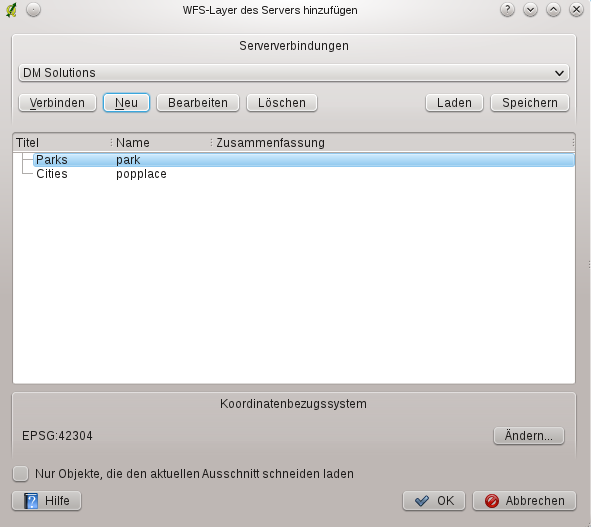
\includegraphics[clip=true,width=0.6\textwidth]{connection_wfs}
  \end{center}
\end{figure}

Se non si attiva la casella di controllo \checkbox{Richiedi solo geometrie in 
sovrapposizione all'estensione della vista attuale}, QGIS acquisisce tutte le
geometrie dal server WFS. Attivando, invece, la casella di controllo, è possibile 
ottenere un sottoinsieme dei dati relativamente alla sola area di proprio interesse.
L'opzione aggiunge alla richiesta al server il parametro BBOX (bounding box) con i valori impostati 
sulla vista attuale: in tal modo si evita di scaricare un intero database. 

Si noti che l'avanzamento della ricezione dei dati viene visualizzato nella
parte inferiore sinistra della finestra principale di QGIS. 
Quando il layer è caricato, è possibile identificare e selezionare alcuni
elementi e visualizzare la tabella attributi.

Il plugin WFS funziona al meglio con server WFS basati su UMN
MapServer. Sono ancora possibili comportamenti anomali e blocchi del plugin,
ma ci saranno miglioramenti in future versioni. Attualmente è supportato WFS
1.0.0: è ancora in fase di test il supporto per altri server WFS. In caso 
di problemi con il plugin, non esitare a contattare il team di sviluppo.
Si veda la Sezione \ref{label_helpsupport} per ulteriori informazioni sulle mailinglist.

\begin{Tip}[ht]\caption{\textsc{Cercare server WFS}}
È possibile ricercare ulteriori server WFS tramite Google o altro
motore di ricerca preferito. Ci sono anche diversi elenchi di URL pubblici,
alcuni dei quali aggiornati e altri non più mantenuti.
\index{WFS!server remoto!}
\end{Tip} 

\FloatBarrier
